

\tikzset{every picture/.style={line width=0.75pt}} %set default line width to 0.75pt        

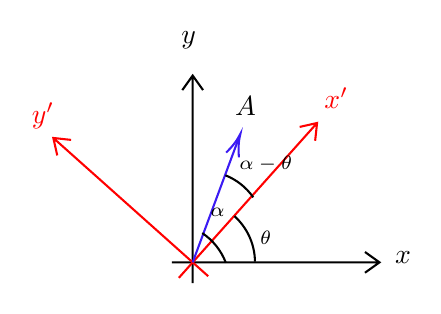
\begin{tikzpicture}[x=0.75pt,y=0.75pt,yscale=-1,xscale=1]
%uncomment if require: \path (0,201); %set diagram left start at 0, and has height of 201

%Shape: Axis 2D [id:dp5999262441064296] 
\draw  (283,150) -- (383,150)(293,60) -- (293,160) (376,145) -- (383,150) -- (376,155) (288,67) -- (293,60) -- (298,67)  ;
%Shape: Axis 2D [id:dp6999025250833045] 
\draw [color={rgb, 255:red, 255; green, 0; blue, 0 }  ,draw opacity=1 ] (286.34,157.46) -- (352.93,82.85)(225.85,90.07) -- (300.46,156.66) (344.54,84.75) -- (352.93,82.85) -- (352,91.41) (227.75,98.46) -- (225.85,90.07) -- (234.41,91)  ;
%Shape: Arc [id:dp9879953663640971] 
\draw  [draw opacity=0][line width=0.75]  (313.11,127.73) .. controls (319.05,133.11) and (322.85,140.84) .. (323,149.49) .. controls (323,149.54) and (323,149.6) .. (323,149.65) -- (293,150) -- cycle ; \draw  [line width=0.75]  (313.11,127.73) .. controls (319.05,133.11) and (322.85,140.84) .. (323,149.49) .. controls (323,149.54) and (323,149.6) .. (323,149.65) ;  
%Straight Lines [id:da08151702925178561] 
\draw [color={rgb, 255:red, 59; green, 27; blue, 243 }  ,draw opacity=1 ]   (293,150) -- (315.3,89.91) ;
\draw [shift={(316,88.03)}, rotate = 110.36] [color={rgb, 255:red, 59; green, 27; blue, 243 }  ,draw opacity=1 ][line width=0.75]    (10.93,-3.29) .. controls (6.95,-1.4) and (3.31,-0.3) .. (0,0) .. controls (3.31,0.3) and (6.95,1.4) .. (10.93,3.29)   ;
%Shape: Arc [id:dp7996887661941752] 
\draw  [draw opacity=0][line width=0.75]  (297.62,135.89) .. controls (302.69,139.3) and (306.73,144.24) .. (308.98,150.2) -- (280.91,160.81) -- cycle ; \draw  [line width=0.75]  (297.62,135.89) .. controls (302.69,139.3) and (306.73,144.24) .. (308.98,150.2) ;  
%Shape: Arc [id:dp8674168141053495] 
\draw  [draw opacity=0][line width=0.75]  (308.79,108.05) .. controls (314.04,110.15) and (318.74,113.75) .. (322.19,118.68) -- (297.62,135.89) -- cycle ; \draw  [line width=0.75]  (308.79,108.05) .. controls (314.04,110.15) and (318.74,113.75) .. (322.19,118.68) ;  

% Text Node
\draw (324,133.4) node [anchor=north west][inner sep=0.75pt]  [font=\scriptsize]  {$\theta $};
% Text Node
\draw (389,143.43) node [anchor=north west][inner sep=0.75pt]    {$x$};
% Text Node
\draw (286,37.43) node [anchor=north west][inner sep=0.75pt]    {$y$};
% Text Node
\draw (355,64.43) node [anchor=north west][inner sep=0.75pt]  [color={rgb, 255:red, 255; green, 0; blue, 0 }  ,opacity=1 ]  {$x'$};
% Text Node
\draw (214,71.43) node [anchor=north west][inner sep=0.75pt]  [color={rgb, 255:red, 255; green, 0; blue, 0 }  ,opacity=1 ]  {$y'$};
% Text Node
\draw (300,122.4) node [anchor=north west][inner sep=0.75pt]  [font=\scriptsize]  {$\alpha $};
% Text Node
\draw (312,68.43) node [anchor=north west][inner sep=0.75pt]    {$A$};
% Text Node
\draw (314,97.4) node [anchor=north west][inner sep=0.75pt]  [font=\scriptsize]  {$\alpha -\theta $};


\end{tikzpicture}
l